% National High School Journal of Science Submission — ANONYMIZED VERSION
% Per NHSJS guidelines: author name, affiliation, acknowledgments removed
% File name: Beyond Accuracy - Investigating Calibration Bootstrap Uncertainty and Fairness Gaps in Machine Learning Classifiers
% Compile: pdflatex manuscript_anonymized.tex (run twice)

\documentclass[12pt]{article}
\usepackage[T1]{fontenc}
\usepackage[margin=1in]{geometry}
\usepackage{times}
\usepackage{amsmath}
\usepackage{booktabs}
\usepackage{graphicx}
\usepackage{caption}
\usepackage{hyperref}
\hypersetup{colorlinks=true,linkcolor=black,citecolor=black,urlcolor=blue}

\usepackage[super,numbers,sort&compress]{natbib}

\captionsetup{font=small, labelfont=bf}

\begin{document}

\begin{center}
{\large \textbf{Beyond Accuracy: Investigating Calibration, Bootstrap
Uncertainty, and Fairness Gaps in Machine Learning Classifiers}}

\vspace{0.5em}
{\small \textit{Keywords:} machine learning; calibration; fairness; AUC;
bootstrap uncertainty; small datasets; classifier evaluation}
\end{center}

\begin{abstract}
Most people evaluating a machine learning model stop at one number: AUC,
the area under the ROC curve. If it clears some threshold---say, 0.75 or
0.80---the model gets called ``good enough'' and the evaluation ends there.
I wanted to find out what that habit actually hides.

I trained three classifiers---Logistic Regression, Random Forest, and
CatBoost---on the IBM HR Analytics Employee Attrition dataset (1,470
employee records) and then ran three checks that AUC never runs for you.
First, I measured calibration: do the model's probability outputs actually
match real outcome rates, or do they just rank things in the right order
while being numerically wrong? I used Expected Calibration Error (ECE)
before and after applying an isotonic regression correction. Second, I built
bootstrap confidence intervals on AUC using 1,000 resamples of the test
set---because any single 294-record test split is just one of many possible
draws, and I wanted to see how much the score would bounce around. Third, I
computed fairness metrics (Demographic Parity Difference and Equalized Odds
Difference) for gender and age groups to check whether prediction errors
fell equally on different groups of people.

The results were more uncomfortable than I expected. All three models
cleared 0.75 AUC. CatBoost's probability outputs were off by 8.6 percentage
points on average before correction. Every model's bootstrap confidence
interval was about 15--16 percentage points wide, meaning a ``0.762 AUC''
could just as plausibly have been 0.68 or 0.84 on a different random split.
The age-group fairness gap reached 0.258 for CatBoost---a 26-point
difference in how errors were distributed between younger and older
employees---while the AUC score showed nothing wrong at all. The point of
this paper is not that these problems are unusual. It's that they showed up
together, in the same ordinary models, without any signal from the metric
everyone relies on.
\end{abstract}

\newpage

\section{Introduction}

When someone calls an AI system ``82\% accurate,'' it sounds reassuring. More
than four out of five predictions right. But I kept running into a question
I couldn't shake while working on this project: what does that number actually
tell you, and what does it leave out?

The more I read about how machine learning classifiers get evaluated in
practice, the more I noticed that the standard metric---AUC, or area under the
receiver operating characteristic curve---says nothing about several things
that seem important. It doesn't say whether the model's confidence scores
(the actual probability numbers it outputs) are trustworthy. It doesn't say
how much the reported score might vary if you happened to use a different
random split of the data. And it says nothing about whether the model makes
worse errors for some groups of people than others.

These gaps might not matter much for a classifier that's sorting emails or
tagging product photos. But when predictions feed into decisions about hiring,
lending, healthcare, or student evaluation---contexts where the model's output
affects real people---a single AUC score seems like a thin basis for claiming
the system works.

AUC measures rank discrimination: given a randomly chosen positive case and a
randomly chosen negative case, what fraction of the time does the model rank
the positive one higher?\textsuperscript{1} An AUC of 0.50 is random chance;
0.80 means the model gets the ranking right 80\% of the time. That's
genuinely useful. But it's a measure of ordering, not calibration. Two models
can have identical AUC while one outputs probabilities that closely track
actual event rates and the other is systematically off by a large margin. If
anyone acts on those probability numbers---which happens regularly---they're
working with two very different tools despite the identical AUC.

Calibration is the property that a model's stated confidence actually matches
the observed outcome rate.\textsuperscript{2} A model that says ``70\%
probability of attrition'' is well-calibrated if roughly 70\% of employees
with that predicted probability actually leave. Expected Calibration Error
(ECE) formalizes this by computing the weighted average gap between predicted
probability and observed frequency across confidence bins.\textsuperscript{3}
Tree-based and boosting models are known to be systematically overconfident:
they push predicted probabilities toward 0 and 1 more aggressively than the
data supports.\textsuperscript{4}

Beyond calibration, any single test-set AUC is one draw from a noisy process.
The 294 examples in my test set are just one possible partition of 1,470
total records. Bootstrap resampling---repeatedly sampling the test set with
replacement and re-evaluating---lets you see how wide the plausible range of
outcomes actually is. A 95\% confidence interval that spans 15 percentage
points is telling you something meaningful about precision that the point
estimate hides.

Finally, a classifier with good average performance can still make
systematically worse predictions for certain demographic groups. Hardt et
al.\ defined two concrete metrics for this: Demographic Parity Difference
(DPD), the gap in positive prediction rates between groups, and Equalized
Odds Difference (EOD), the gap in error structure (true positive and false
positive rates) between groups.\textsuperscript{5} A growing literature
documents that trained models frequently exhibit disparate behavior across
race, gender, and age even when overall performance looks
acceptable.\textsuperscript{6}

I wanted to test all of this on a small dataset with standard tools. The goal
wasn't to build the best model. It was to find out whether the hidden gaps
are actually detectable---and whether AUC would have caught them if I hadn't
looked.

\section{Methods}

\subsection{Dataset}

I used the IBM HR Analytics Employee Attrition dataset, a synthetic
organizational benchmark publicly available through
Kaggle.\textsuperscript{7} It contains 1,470 employee records described by
35 variables including job characteristics, satisfaction ratings,
demographics, and compensation. The binary outcome is attrition (employee
departure); 241 of 1,470 records (16.1\%) are labeled positive.

The dataset is synthetic---generated by IBM for educational purposes, not
derived from a real workforce. This is a meaningful limitation: the results
describe model behavior on a simulated benchmark, and patterns like the
age-group fairness gap may reflect how the data was generated rather than
generalizing to real organizations. I chose it because it is publicly
available, reproducible, and free of privacy concerns.

Data were split 80/20 (training: 1,176 records, test: 294) using stratified
sampling to preserve the 16.1\% positive rate in both sets.

\subsection{Classifiers}

Three classifiers were trained:
\begin{enumerate}
  \item \textbf{Logistic Regression (LR)}: a linear model that produces
    calibrated probabilities under well-specified conditions, used as a
    calibration baseline.
  \item \textbf{Random Forest (RF)}: an ensemble of decision trees, widely
    used in practice on tabular data.\textsuperscript{8}
  \item \textbf{CatBoost (CB)}: a gradient boosting algorithm with native
    categorical handling.\textsuperscript{9}
\end{enumerate}

No hyperparameter tuning was performed. The goal was to observe how these
classifiers look under extended evaluation at representative performance
levels, not to maximize AUC.

\subsection{Evaluation Protocol}

Four evaluation components were applied to each model:
\begin{enumerate}
  \item \textbf{AUC} on the held-out test set.
  \item \textbf{Expected Calibration Error (ECE)} before and after post-hoc
    correction using isotonic regression fitted on a held-out calibration
    split (20\% of the training set).
  \item \textbf{Bootstrap confidence intervals} on AUC: 1,000 resamples
    of the test set with replacement, reporting the 2.5th--97.5th percentile
    interval.
  \item \textbf{Fairness metrics} (DPD and EOD) for gender (Male vs.\
    Female) and age group (under 40 vs.\ over 40) using CatBoost predictions
    and a 0.5 decision threshold.
\end{enumerate}

All code is available at: https://github.com/SilverCoin256/accuracy-isnt-enough

\section{Results}

\subsection{AUC}

All three models achieved AUC scores in the 0.76--0.80 range (Table 1).
Logistic Regression came out highest at 0.798, which was a little
unexpected---simpler models don't always outperform ensembles on tabular
data. All three scores are meaningfully above the 0.50 random baseline.
Stopping the evaluation here, everything would look fine.

\begin{table}[htbp]
\centering
\caption{Test-set AUC for each classifier.}
\label{tab:auc}
\begin{tabular}{lc}
\toprule
\textbf{Model} & \textbf{AUC} \\
\midrule
Logistic Regression & 0.798 \\
Random Forest       & 0.759 \\
CatBoost            & 0.762 \\
\bottomrule
\end{tabular}
\end{table}

\subsection{Calibration}

Table 2 shows ECE before and after isotonic regression correction.

\begin{table}[htbp]
\centering
\caption{Expected Calibration Error before and after isotonic regression
correction.}
\label{tab:ece}
\begin{tabular}{lcc}
\toprule
\textbf{Model} & \textbf{ECE (before)} & \textbf{ECE (after)} \\
\midrule
Logistic Regression & 0.047 & 0.058 \\
Random Forest       & 0.032 & 0.036 \\
CatBoost            & 0.086 & 0.066 \\
\bottomrule
\end{tabular}
\end{table}

CatBoost's pre-calibration ECE was 8.6\%---its probability outputs deviated
from actual outcome rates by about 9 percentage points on average.
The reliability diagram (Figure 1) shows the shape of this miscalibration:
the model's predictions cluster above the perfect-calibration diagonal at
the high-confidence end, claiming more certainty than the data supports.

What I didn't expect: Logistic Regression's ECE got slightly \textit{worse}
after correction, from 0.047 to 0.058. LR has theoretical calibration
properties under certain conditions, so applying isotonic regression to it
apparently introduced noise rather than improvement. My best explanation is
that the calibration fitting set was too small (around 200 examples) to
reliably estimate a correction for a model that was already fairly well
calibrated. CatBoost improved the most, from 0.086 to 0.066---a 23\%
reduction---consistent with the known overconfidence of boosting models.

\begin{figure}[htbp]
\centering
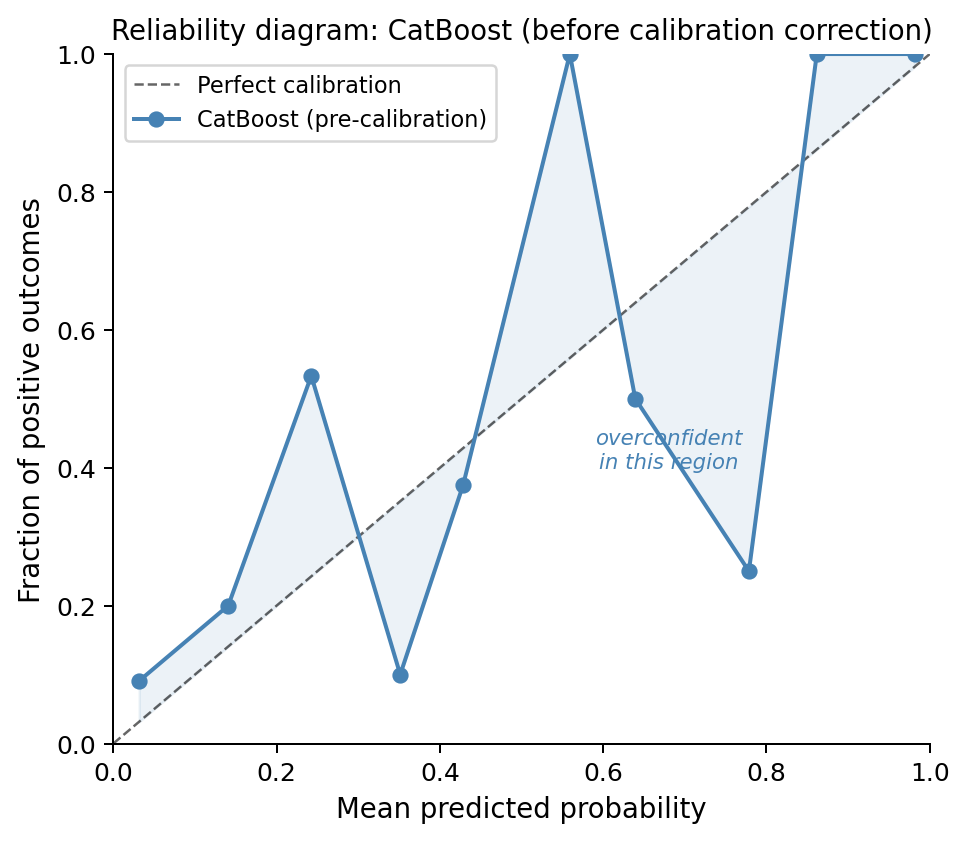
\includegraphics[width=0.70\textwidth]{figures/fig1_reliability_diagram.png}
\caption{Reliability diagram for CatBoost before calibration correction.
  The dashed diagonal is perfect calibration. The model's predictions
  fall above the diagonal at high confidence levels, indicating
  overconfidence in the region where predictions are most likely to
  drive decisions.}
\label{fig:calibration}
\end{figure}

\subsection{Bootstrap Confidence Intervals}

Table 3 shows 95\% bootstrap confidence intervals on AUC for each model.

\begin{table}[htbp]
\centering
\caption{Bootstrap 95\% confidence intervals on AUC (1,000 resamples).}
\label{tab:bootstrap}
\begin{tabular}{lccc}
\toprule
\textbf{Model} & \textbf{AUC} & \textbf{95\% CI} & \textbf{Width} \\
\midrule
Logistic Regression & 0.798 & [0.716, 0.874] & 0.158 \\
Random Forest       & 0.759 & [0.686, 0.832] & 0.146 \\
CatBoost            & 0.762 & [0.676, 0.838] & 0.162 \\
\bottomrule
\end{tabular}
\end{table}

Every model's interval is roughly 15--16 percentage points wide. CatBoost's
interval runs from 0.676 to 0.838---meaning the same model and pipeline
could plausibly have reported any AUC in that range depending on which 294
records ended up in the test set. The point estimate of 0.762 is one draw
out of many possible draws.

This result bothered me more than the calibration issue. Calibration error
has a known correction; these confidence intervals don't have a fix. They are
just an honest description of what 1,470 records can and can't tell you.
Reporting only the point estimate, without this context, is technically
accurate but creates a false impression of precision.

Figure 2 shows the bootstrap distribution for CatBoost.

\begin{figure}[htbp]
\centering
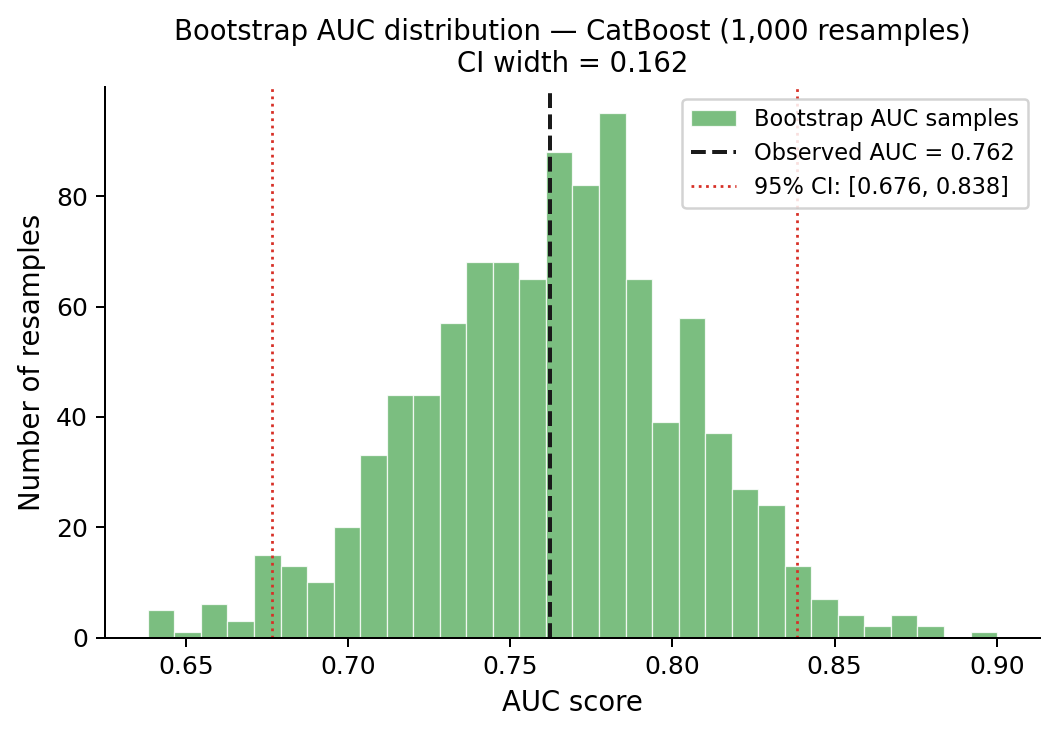
\includegraphics[width=0.72\textwidth]{figures/fig2_bootstrap_distribution.png}
\caption{Bootstrap distribution of CatBoost AUC scores across 1,000
  resamples. The dashed line is the observed test-set AUC. The red
  dotted lines mark the 95\% confidence interval boundaries.
  The spread illustrates the sensitivity of any single-split evaluation
  on a dataset of this size.}
\label{fig:bootstrap}
\end{figure}

\subsection{Fairness Metrics}

Table 4 shows DPD and EOD for gender and age group using CatBoost predictions.

\begin{table}[htbp]
\centering
\caption{Fairness metrics for CatBoost. DPD = Demographic Parity
  Difference; EOD = Equalized Odds Difference. Lower is better.}
\label{tab:fairness}
\begin{tabular}{lcc}
\toprule
\textbf{Group} & \textbf{DPD} & \textbf{EOD} \\
\midrule
Gender (Male vs.\ Female) & 0.018 & 0.026 \\
Age (Under 40 vs.\ Over 40)   & 0.062 & 0.258 \\
\bottomrule
\end{tabular}
\end{table}

Gender disparity was small on both metrics. The age disparity was not.
An EOD of 0.258 means there was a 26-percentage-point gap in the error
structure between younger and older employee groups, despite the identical
aggregate AUC for both.

Interpreting this on a synthetic dataset requires caution: the pattern may
reflect how IBM constructed the simulation rather than something that
generalizes. But the gap showed up regardless, and it is exactly the kind of
finding that AUC does not surface. Figure 3 shows the comparison.

\begin{figure}[htbp]
\centering
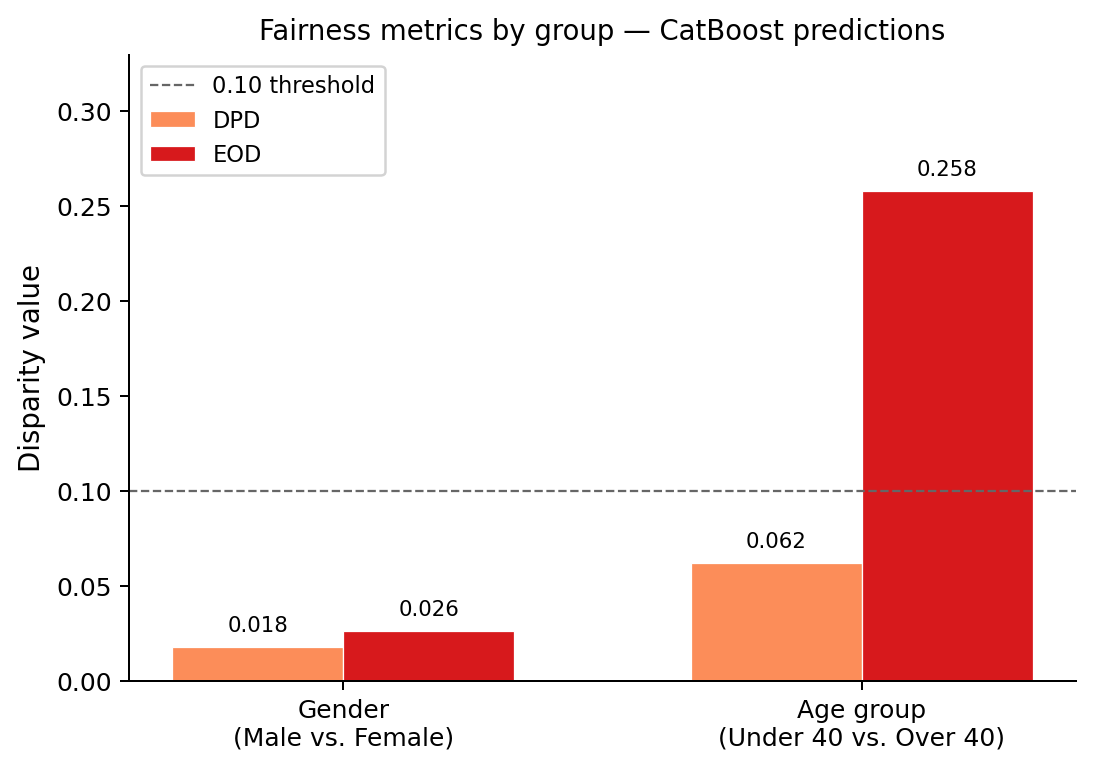
\includegraphics[width=0.65\textwidth]{figures/fig3_fairness_comparison.png}
\caption{Equalized Odds Difference and Demographic Parity Difference by
  demographic group, using CatBoost predictions. The dashed reference
  line at 0.10 marks a commonly cited threshold for acceptable disparity.
  The age-group EOD of 0.258 substantially exceeds this threshold.}
\label{fig:fairness}
\end{figure}

\section{Discussion}

\textbf{Three problems, one model, one dataset.}
What struck me reviewing these results is how the three problems appeared
together. I expected some calibration error from CatBoost---that's
well-documented. I expected fairly wide bootstrap intervals on a small
dataset. The age-group fairness gap was larger than I anticipated. But finding
all three at once, in the same models, while the AUC scores looked perfectly
acceptable---that was the part I kept turning over. None of these are exotic
failure modes. They showed up on a standard benchmark using default
hyperparameters.

\textbf{Small datasets.}
Part of the story is sample size. With 1,470 records and 294 test examples,
the evaluation is inherently noisy. Wider bootstrap intervals, noisier
calibration corrections, less stable fairness metrics across demographic
subgroups---these are all predictable consequences of having limited data. The
less comfortable part: 1,470 records is not unusual for many real deployment
settings. School districts, community healthcare organizations, small
municipalities---these are exactly the places where AI tools are being
adopted, and their datasets are often this size or smaller.

\textbf{Calibration correction is not automatic.}
Post-hoc calibration improved CatBoost (ECE down 23\%) and Random Forest
(marginal improvement). It made Logistic Regression slightly worse. This is
a reminder that calibration correction requires holding back data to fit
the correction layer, and on small datasets the fitting can be noisy. It is
not a guaranteed win.

\textbf{What I'd do differently.}
The clearest limitation is the synthetic dataset. I chose it for
reproducibility and accessibility, but it means the age-group fairness gap
might be an artifact of how the simulation was constructed. The necessary
next step would be running the same evaluation on a real organizational
dataset with verified demographic variation.

I also want to know whether the age-group EOD shrinks after calibration
correction. CatBoost was the most miscalibrated model and also the most
fairness-disparate. Those might be connected: if the overconfidence is
unevenly distributed across age groups, correcting the calibration might
also reduce the fairness gap. I didn't check this here because the
correction didn't produce clean results across all models, but it's the
question I'm most curious about from this work.

\section{Conclusion}

I started this project wondering whether AUC was genuinely sufficient for
evaluating machine learning classifiers, or whether it was just the metric
everyone defaulted to because it was convenient. The answer on this dataset
is that it misses real things---calibration error, uncertainty in the
estimate itself, and demographic fairness gaps---that show up clearly with
a few additional standard tools.

None of the additional metrics I used are obscure. ECE, bootstrap confidence
intervals, DPD, and EOD are all implemented in scikit-learn and can be added
to an existing evaluation pipeline in a few hours. The return on that
investment, based on what I found here, is a substantially more complete
picture of what the model is and isn't doing.

A single AUC score passing some threshold is not the same as a model being
ready to be trusted in a context where predictions affect people. The three
models I evaluated cleared the AUC bar while failing the calibration,
stability, and fairness checks. Whether those failures matter depends on
the application---but the point is that you have to check. There's a broader
argument in the literature that uncritical reliance on convenient metrics
accumulates into serious deployment problems downstream.\textsuperscript{10}
This is a small illustration of why.

\section*{References}
\sloppy
\begin{enumerate}
\item T. Fawcett. An introduction to ROC analysis. Pattern Recognition
  Letters. Vol. 27, pg. 861--874, 2006,
  https://doi.org/10.1016/j.patrec.2005.10.010.

\item J. DeGrave, J. Janizek, S. Lee. AI for radiographic COVID-19 detection
  selects shortcuts over signal. Nature Machine Intelligence. Vol. 3,
  pg. 610--619, 2021, https://doi.org/10.1038/s42256-021-00338-7.

\item C. Guo, G. Pleiss, Y. Sun, K. Q. Weinberger. On calibration of modern
  neural networks. Proceedings of the 34th International Conference on
  Machine Learning. Vol. 70, pg. 1321--1330, 2017,
  http://proceedings.mlr.press/v70/guo17a.html.

\item A. Niculescu-Mizil, R. Caruana. Predicting good probabilities with
  supervised learning. Proceedings of the 22nd International Conference on
  Machine Learning. pg. 625--632, 2005,
  https://doi.org/10.1145/1102351.1102430.

\item M. Hardt, E. Price, N. Srebro. Equality of opportunity in supervised
  learning. Advances in Neural Information Processing Systems. Vol. 29,
  pg. 3323--3331, 2016,
  https://proceedings.neurips.cc/paper/2016/hash/9d2682367c3935defcb1f9e247a97c0d-Abstract.html.

\item N. Mehrabi, F. Morstatter, N. Saxena, K. Lerman, A. Galstyan.
  A survey on bias and fairness in machine learning. ACM Computing Surveys.
  Vol. 54, pg. 1--35, 2021, https://doi.org/10.1145/3457607.

\item IBM Data Scientists. IBM HR analytics employee attrition \&
  performance [synthetic dataset]. Kaggle, 2015,
  https://www.kaggle.com/datasets/pavansubhasht/ibm-hr-analytics-attrition-dataset.

\item L. Breiman. Random forests. Machine Learning. Vol. 45, pg. 5--32,
  2001, https://doi.org/10.1023/A:1010933404324.

\item L. Prokhorenkova, G. Gusev, A. Vorobev, A. V. Dorogush, A. Gulin.
  CatBoost: unbiased boosting with categorical features. Advances in
  Neural Information Processing Systems. Vol. 31, 2018,
  https://proceedings.neurips.cc/paper/2018/hash/14491b756b3a51daac41c24863285549-Abstract.html.

\item D. Sculley, G. Holt, D. Golovin, E. Davydov, T. Phillips, D. Ebner,
  V. Chaudhary, M. Young, J. Crespo, D. Dennison. Hidden technical debt
  in machine learning systems. Advances in Neural Information Processing
  Systems. Vol. 28, pg. 2503--2511, 2015,
  https://proceedings.neurips.cc/paper/2015/hash/86df7dcfd896fcaf2674f757a2463eba-Abstract.html.

\end{enumerate}

\end{document}
